\subsection{Common Kubernetes infrastructure for all Web Frameworks}
\label{sec-web-frameworks}

\begin{table}[h!]
\begin{tabularx}{\textwidth}{ p{10em}| >{\raggedright\arraybackslash}X}
    \emph{Name} & \emph{Indicative use case} \\
    \hline \\
    EOS web hosting & Serve static HTML/CSS/JS/CGI stored on the EOS shared filesystem with simple deployment requirements \\
    Platform as a Service (PaaS) & Custom web applications with flexible deployment on Openshift (Kubernetes) \\
    CMS/Drupal & Websites for visual site building (see sec. \ref{what-is-drupal}) \\
    Discourse & A home for communities around a common topic \\
    TWiki & Wiki format content creation platform
\end{tabularx}
\caption{\emph{Web Frameworks}: web hosting and content creation platforms based on different technologies.
EOS web hosting and PaaS are \emph{already using the common Kubernetes infrastructure}.}
\vspace{-1.8em}
\label{tab-wf}
\end{table}

For each web framework there is currently a separate infrastructure, based on different technologies.
This creates silos of operational expertise within the small engineering team that supports each one, which are \emph{costly and inefficient} to keep alive in CERN's dynamic working environment.
At the same time, there are a lot of software components developed in-house to support a single use case at the time, generating a large technical debt.
Many requirements however are shared, such as interfacing with external CERN systems.

\begin{wrapfigure}{r}{.62\textwidth}
    \vspace{-1em}
    \centering
    \hspace{-1.8em}
    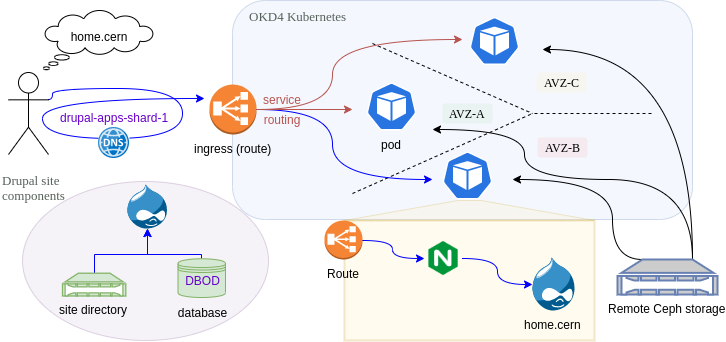
\includegraphics[width=.66\textwidth]{figures/drupal-k8s-request-journey}
    \caption{\emph{Request journey through the Kubernetes infrastructure}. Contrast with figure \ref{fig:drupal-physical-request-journey}.}
    \vspace{-2em}
    \label{fig:drupal-k8s-request-journey}
\end{wrapfigure}

We therefore developed a common platform on the \emph{Openshift Kubernetes community distribution (OKD 4)},
leaving only a thin business logic layer specific to each use case.
OpenShift was chosen firstly for its production-tested multitenancy support, which we relied on for the present PaaS infrastructure.
Openshift extends Kubernetes with tooling that simplifies our design \cite{jarvinenExtendingKubernetesOperator2019}:
a developer-focused console UI that we expose to end users, in-place upgrades of the control plane, node (machine) management API, monitoring and logging stacks.

The first web frameworks to use the new infrastructure are EOS web hosting (in production since \emph{November 2020},
and PaaS (in production since \emph{March 2021}).
The Drupal use case is in Pilot phase, due to enter production in summer 2021.

\subsection{Serving perspective}

The physical servers are replaced with virtual machines composing an OKD 4 cluster.
Each website is served by 1 or multiple replicas of a pod with Nginx and PHP-FPM containers,
in different cloud availability zones in case of critical websites.
The server perspective can be seen by following an HTTP request in figure \ref{fig:drupal-k8s-request-journey}.

\subsection{DrupalSite API: create and manage websites}

\begin{figure}[t]
    \centering
    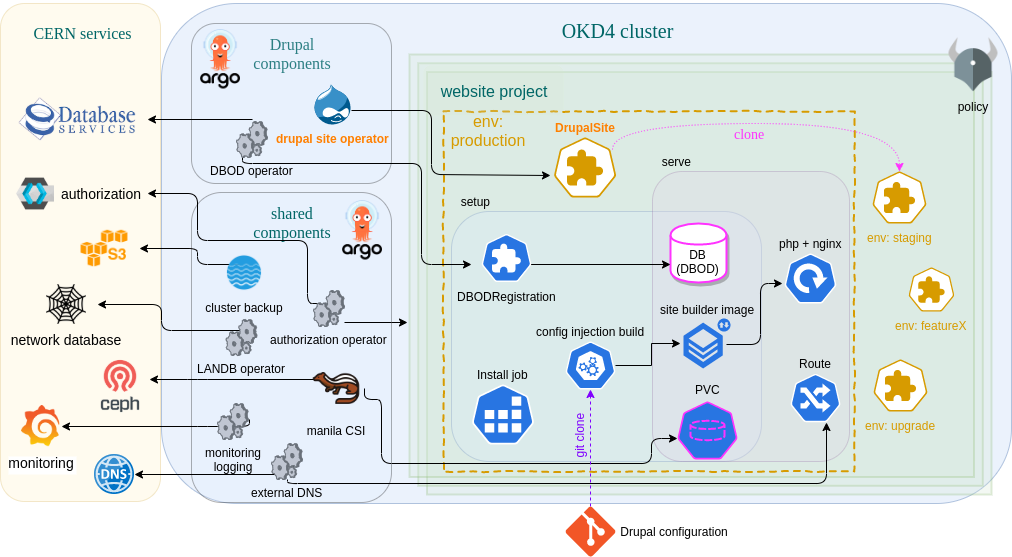
\includegraphics[width=.95\textwidth]{figures/drupal-architecture}
    \vspace{-1em}
    \caption{\emph{Drupal cluster architecture}.
    The diagram presents the \emph{Kubernetes resources} that {\color{darkseagreen} make up a Drupal site},
    the {\color{carolinablue} controllers} that manage them and the cluster infrastructure,
    and the {\color{beige} external CERN systems} with which the cluster integrates.
    Policy is handled with Open Policy Agent \cite{openPolicyAgent}.
    The {\color{fluorescentorange} DrupalSite CRD} is an API for website definition.
    The components are deployed with Helm \cite{helmsh} and maintained with ArgoCD \cite{argocd}}
    \label{fig:drupal-architecture}
    \vspace{-2em}
\end{figure}

The infrastructure can be seen as an application that offers its users functions to manage websites.
It provides an API for website admins to specify the kind of website they need: what version of Drupal, what amount of resources, which git repository to fetch configuration from.
Each \texttt{Project} (Kubernetes namespace) forms the administrative domain of a website: it serves a single production website.
Website admins can similarly create different \emph{environments} of their website in the same project for development or test purposes (which are full websites with independent data stores),
clone data between websites, and take and restore backups.
An overview of the components is in figure \ref{fig:drupal-architecture}.

Following the operator pattern introduced in section \ref{sec-operators}, the business logic is implemented with the \emph{\texttt{DrupalSite} Custom Resource Definition} (CRD) and the \emph{drupalSite operator}.
The \texttt{DrupalSite}, in turn, controls all the resources in the { \color{fluorescentorange} dashed box } in the architecture diagram (figure \ref{fig:drupal-architecture}).

Each website runs an immutable version of Drupal code, compiled from a version of the \href{https://gitlab.cern.ch/drupal/paas/cern-drupal-distribution/}{CERN Drupal distribution}
(controlled by the Infrastructure team) with a source-to-image build that injects user dependencies and configuration from a git repository.
Site administrators with technical background thus gain extra flexibility in customizing their website.

%- admin workflow to update Drupal version
%\subsubsection{Upgrading Drupal version}

We describe \emph{more technical details of the Operator in \cite{kubeconCernOperators}}.